% Provenance (never printed): see sources/outline_sources.md (Year 1: optical
% mineralogy with the polarising microscope; Michel-Levy chart). Interference
% colours in figdata/bachelor-1/michel_levy.py from the CIE 1931 colour-matching
% functions and illuminant D65 (data/derived/bachelor-1-cie*.csv); exercise and
% problem values in the Book 3 scratch calculator calc/ch08.py.
\chapter{علم المعادن البصري}\label{ch:b1:optical-mineralogy}

بين \omterm{def:b1:field-lab-methods-1:microscope}{المستقطِبين المتقاطعين} تُضيء \omterm{def:b1:field-lab-methods-1:thin-section}{الشريحة الرقيقة} من الغابرو كزجاج ملوّن. تعبر المجال شرائح طويلة رمادية وبيضاء، مخطّطة كالشفرة الشريطية؛ وبينها تتوهّج حبيبات زرقاء وصفراء وأرجوانية؛ وتبقى قلّة منها سوداء مهما دارت. ولكل من هذه الظواهر سبب يمكن حسابه، وكل منها يدل على \omterm{def:b1:rock-forming-minerals:mineral}{المعدن} الموجود. يشرح هذا الفصل كيف يعبر الضوء البلورة، ولماذا يكون \omterm{def:b1:rock-forming-minerals:mineral}{المعدن} بين \omterm{def:b1:field-lab-methods-1:microscope}{المستقطِبين المتقاطعين} ملوّنًا، وكيف يقيس اللون خاصية من خواص \omterm{def:b1:rock-forming-minerals:mineral}{المعدن}، وكيف يسمّي عالِم الصخور حبيبات \omterm{def:b1:field-lab-methods-1:thin-section}{الشريحة الرقيقة} بالمجهر وحده. ويختم بشريحة مجهولة تُستخلص معادنها وسمكها الحقيقي مما تُريه.

\begin{recall}
\omterm{def:b1:field-lab-methods-1:thin-section}{الشريحة الرقيقة} شريحة صخر بسمك نحو \qty{30}{\micro m} على شريحة زجاجية؛ ويفحصها \omterm{def:b1:field-lab-methods-1:microscope}{المجهر المستقطِب} في \omterm{def:b1:field-lab-methods-1:microscope}{الضوء المستقطَب المستوي} (مستقطِب واحد) وبين \omterm{def:b1:field-lab-methods-1:microscope}{المستقطِبين المتقاطعين} (\cref{ch:b1:field-lab-methods-1}). معامل الانكسار $n$ لوسط هو نسبة سرعة الضوء في الفراغ إلى سرعته في الوسط، والانكسار عند سطح فاصل يخضع لقانون سنل $n_1\sin i_1 = n_2\sin i_2$ (من كتاب الفيزياء للسنة الأولى). الضوء موجة مستعرضة؛ والمستقطِب لا يمرّر إلا مركبة المجال الكهربائي على اتجاهه، فيمرّر محلّل يميل بزاوية $\alpha$ عليه الكسر $\cos^2\alpha$ من الشدة (قانون مالوس، من كتب الفيزياء).
\end{recall}

\section{الضوء في البلورات}

في الزجاج أو السائل أو البلورة المكعّبة، يسير الضوء بالسرعة نفسها في كل اتجاه ومهما كان اتجاه اهتزازه. أما في معظم \omterm{def:b1:rock-forming-minerals:mineral}{المعادن} فلا: ترتيب الذرات يختلف باختلاف الاتجاهات، وكذلك استجابة الإلكترونات للمجال الكهربائي للموجة.

\begin{definition}[المعادن متساوية الخواص ومتباينة الخواص]\label{def:b1:optical-mineralogy:anisotropic}
\omterm{def:b1:rock-forming-minerals:mineral}{المعدن} \emph{متساوي الخواص}\index{معدن متساوي الخواص} حين يكون معامل انكساره نفسه لكل اتجاه انتشار واهتزاز للضوء؛ \omterm{def:b1:rock-forming-minerals:mineral}{والمعادن} المكعّبة (\omterm{def:b1:rock-forming-minerals:groups}{الجارنيت}، والهاليت، والسبينل) والزجاج متساوية الخواص. وهو \emph{متباين الخواص}\index{معدن متباين الخواص} حين يتوقف معامل انكساره على اتجاه الاهتزاز؛ وكل \omterm{def:b1:rock-forming-minerals:mineral}{معادن} المجموعات البلورية الأخرى متباينة الخواص.
\end{definition}

لا تعبر شريحة مقطوعة من بلورة متباينة الخواص الضوء كموجة واحدة. نقبل النتيجة التالية من بصريات البلورات (من كتاب الفيزياء للسنة الثانية): لاتجاه انتشار معلوم، تنقل شريحة من \omterm{def:b1:optical-mineralogy:anisotropic}{المعدن متباين الخواص} موجتين تهتزان في اتجاهين متعامدين ثابتين في الشريحة، هما \emph{اتجاها الاهتزاز}، وتسيران بمعاملي انكسار مختلفين $n_1$ و$n_2$. الضوء المهتز على أحد هذين الاتجاهين يعبر الشريحة دون أن يتغيّر استقطابه؛ أما الضوء المهتز على أي اتجاه آخر فيتفرّق إلى مركبتيه على طوليهما. ويتعلّق المعاملان باتجاه الانتشار، وهناك اتجاهات خاصة يتساويان فيها.

\begin{definition}[المحور البصري، والمعادن أحادية المحور وثنائية المحور]\label{def:b1:optical-mineralogy:optic-axis}
\emph{المحور البصري}\index{المحور البصري} \omterm{def:b1:optical-mineralogy:anisotropic}{لمعدن متباين الخواص} هو اتجاه انتشار يسير فيه الضوء بمعامل انكسار واحد، مهما كان اتجاه اهتزازه، كما في وسط \omterm{def:b1:optical-mineralogy:anisotropic}{متساوي الخواص}. يكون \omterm{def:b1:rock-forming-minerals:mineral}{المعدن} \emph{أحادي المحور}\index{أحادي المحور} حين يملك محورًا بصريًا واحدًا (\omterm{def:b1:rock-forming-minerals:mineral}{معادن} الجمل الثلاثية والرباعية والسداسية، كالكوارتز والكالسيت)، و\emph{ثنائي المحور}\index{ثنائي المحور} حين يملك اثنين (\omterm{def:b1:rock-forming-minerals:mineral}{المعادن} المعينية القائمة والأحادية الميل والثلاثية الميل، \omterm{def:b1:rock-forming-minerals:groups}{كالأوليفين} والبيروكسينات والأمفيبولات \omterm{def:b1:rock-forming-minerals:groups}{والميكا} والفلسبارات).
\end{definition}

تُلخَّص الهندسة بسطح هو المؤشِّرة: مجسّم ناقصي (إهليلجي) نصف قطره في كل اتجاه هو معامل انكسار الضوء المهتز في ذلك الاتجاه. ومقطع المجسّم العمودي على اتجاه الانتشار قطع ناقص محاوره هي اتجاها الاهتزاز، وأنصاف محاوره $n_1$ و$n_2$. وفي \omterm{def:b1:rock-forming-minerals:mineral}{المعدن} \omterm{def:b1:optical-mineralogy:optic-axis}{أحادي المحور} يكون المجسّم مجسّم دوران حول \omterm{def:b1:optical-mineralogy:optic-axis}{المحور البصري}، بمعاملين رئيسيين $n_\omega$ و$n_\varepsilon$: الكوارتز له $n_\omega = 1.544$ و$n_\varepsilon = 1.553$، والكالسيت $1.658$ و$1.486$.
% ledger: hom:quartz-optics, hom:calcite-optics
ولمعدن \omterm{def:b1:optical-mineralogy:optic-axis}{ثنائي المحور} ثلاثة معاملات انكسار رئيسية $n_\alpha < n_\beta < n_\gamma$، ومقطعان دائريان عموديان على محوريه البصريين: للفورستيريت $1.635$ و$1.651$ و$1.670$.
% ledger: hom:forsterite-optics

\begin{definition}[الانكسار المزدوج (للمعدن)]\label{def:b1:optical-mineralogy:birefringence}
\emph{الانكسار المزدوج}\index{الانكسار المزدوج (للمعدن)} \omterm{def:b1:rock-forming-minerals:mineral}{لمعدن} هو الفرق $\delta = n_{\max} - n_{\min}$ بين أكبر معاملي انكساره الرئيسيين وأصغرهما: $n_\varepsilon - n_\omega$ بالقيمة المطلقة \omterm{def:b1:rock-forming-minerals:mineral}{لمعدن} \omterm{def:b1:optical-mineralogy:optic-axis}{أحادي المحور}، و$n_\gamma - n_\alpha$ \omterm{def:b1:rock-forming-minerals:mineral}{لمعدن} \omterm{def:b1:optical-mineralogy:optic-axis}{ثنائي المحور}. وفي حبيبة مقطوعة في أي اتجاه آخر، يقع الفرق $|n_1 - n_2|$ بين 0 (مقطع عمودي على \omterm{def:b1:optical-mineralogy:optic-axis}{المحور البصري}) و$\delta$ (مقطع يحوي اتجاهي $n_{\max}$ و$n_{\min}$).
\end{definition}

\omterm{def:b1:optical-mineralogy:birefringence}{الانكسار المزدوج} خاصية \omterm{def:b1:rock-forming-minerals:mineral}{للمعدن}، شأنه شأن كثافته: الكوارتز \num{0.009}، والكالسيت \num{0.172}، والفورستيريت \num{0.035}، والفايالايت \num{0.052}. وتقطع \omterm{def:b1:field-lab-methods-1:thin-section}{الشريحة الرقيقة} حبيبات \omterm{def:b1:rock-forming-minerals:mineral}{المعدن} في كل اتجاه، فتُظهر حبيباته كل قيمة من 0 إلى $\delta$؛ والقيمة العليا وحدها هي المميّزة.
% ledger: hom:quartz-optics, hom:calcite-optics, hom:forsterite-optics, hom:fayalite-optics

\section{الملاحظات في الضوء المستقطَب المستوي}

بالمستقطِب السفلي وحده يُظهر المجهر شكل الحبيبات ولونها وانشقاقاتها \omterm{def:b1:optical-mineralogy:relief}{والبروز}.

\begin{definition}[تعدّد الألوان الضوئي]\label{def:b1:optical-mineralogy:pleochroism}
يكون \omterm{def:b1:rock-forming-minerals:mineral}{المعدن} \emph{متعدد الألوان}\index{تعدد الألوان الضوئي} حين يتغيّر لونه، مرئيًّا في \omterm{def:b1:field-lab-methods-1:microscope}{الضوء المستقطَب المستوي}، مع دوران المنضدة؛ و\emph{تعدّد الألوان} هو هذا التغيّر. وينشأ من أن امتصاص الضوء يتوقف على اتجاه اهتزازه في البلورة.
\end{definition}

البيوتيت هو المثال الكلاسيكي: حبيبة مقطوعة عبر انشقاقها تنتقل من بنّي مصفرّ شاحب إلى بنّي داكن عند دورانها، وتكون أشدّ قتامة حين تقع آثار الانشقاق على امتداد المستقطِب. والهورنبلند ينتقل من الأصفر إلى الأخضر. وأغلب سيليكات الصخور الأخرى (الكوارتز، والفلسبارات، \omterm{def:b1:rock-forming-minerals:groups}{والأوليفين}، والديوبسيد، والمسكوفيت) عديمة اللون في \omterm{def:b1:field-lab-methods-1:thin-section}{الشريحة الرقيقة}، وتُميَّز حبيباتها عديمة اللون بوسائل أخرى.
% ledger: hom:biotite-optics, hom:hornblende-optics, hom:muscovite-optics, hom:diopside-optics, hom:forsterite-optics

\begin{definition}[البروز، وخط بيك]\label{def:b1:optical-mineralogy:relief}
\emph{البروز}\index{البروز (البصري)} لحبيبة في \omterm{def:b1:field-lab-methods-1:thin-section}{الشريحة الرقيقة} هو مدى وضوح حدودها وشقوقها وسطحها بالنسبة إلى وسط التثبيت؛ ويكون مرتفعًا حين يختلف معامل انكسار الحبيبة ومعامل الوسط كثيرًا، ومنخفضًا حين يتقاربان. و\emph{خط بيك}\index{خط بيك} هو الخط المضيء الرفيع الذي يحدّ حبيبةً يختلف معامل انكسارها عن معامل محيطها حين يخرج المجهر عن البؤرة قليلًا.
\end{definition}

\begin{proposition}[البروز ومعامل الانكسار]\label{prop:b1:optical-mineralogy:relief}
شعاع يعبر بزاوية سقوط $i$ سطحًا فاصلًا بين وسط تثبيت معامله $n_m$ وحبيبة معامل انكسارها $n$ قريب من $n_m$ ينحرف بمقدار
\[
  \varepsilon \approx \frac{|n - n_m|}{n_m}\,\tan i
\]
(بالراديان)، من الرتبة الأولى في $(n - n_m)/n_m$. وتزداد الانحرافات عند الحواف المائلة للحبيبة، ومن ثمّ بروزها، بنسبة $|n - n_m|$.
\end{proposition}

\begin{proof}
يعطي قانون سنل $n_m \sin i = n \sin r$. نكتب $n = n_m(1 + \eta)$ مع $\eta$ صغير، و$r = i - \varepsilon$ مع $\varepsilon$ صغير. إذن
$\sin i = (1 + \eta)(\sin i - \varepsilon\cos i) + O(\eta^2, \varepsilon^2)$،
فيكون $\eta \sin i = \varepsilon\cos i$ من الرتبة الأولى، أي
$\varepsilon = \eta\tan i$، مع $|\eta| = |n - n_m|/n_m$.
\end{proof}

تُثبَّت \omterm{def:b1:field-lab-methods-1:thin-section}{الشريحة الرقيقة} في راتنج معامله نحو $1.54$.
% ledger: jaic:epoxy-ri
يكاد الكوارتز ($1.544$--$1.553$) والفلسبارات ($1.52$--$1.59$) تختفي أمام هذا الوسط: بروز منخفض، وحدود الحبيبات يصعب رؤيتها. أما \omterm{def:b1:rock-forming-minerals:groups}{الأوليفين} ($1.64$--$1.88$) والبيروكسينات والأمفيبولات فتبرز بحواف داكنة وسطح يبدو خشنًا: بروز مرتفع. \omterm{def:b1:rock-forming-minerals:groups}{والجارنيت} ($1.83$) يبدو محاطًا بحافة شبه سوداء. والكالسيت، الذي يتراوح معامل انكساره بين $1.486$ و$1.658$ حسب اتجاه الاهتزاز، يغيّر بروزه عند دوران المنضدة، وهي ظاهرة تُسمّى الوميض.
% ledger: hom:quartz-optics, hom:albite-optics, hom:anorthite-optics, hom:orthoclase-optics, hom:forsterite-optics, hom:fayalite-optics, hom:almandine-optics, hom:calcite-optics
لا يدل \omterm{def:b1:optical-mineralogy:relief}{البروز} إلا على مدى بُعد $n$ عن $n_m$، لا على جهة هذا البُعد؛ أما \omterm{def:b1:optical-mineralogy:relief}{خط بيك} فيدل على الجهة.

\begin{method}[اختبار خط بيك]\label{met:b1:optical-mineralogy:becke}
ركّز على حافة حبيبة في \omterm{def:b1:field-lab-methods-1:microscope}{الضوء المستقطَب المستوي}، واقفل قليلًا الحجاب الحاجز للفتحة، وارفع البؤرة قليلًا (أبعد العدسة الشيئية عن الشريحة). يتحرك الخط المضيء لبيك نحو الوسط ذي معامل الانكسار الأعلى: فإن تحرك نحو الحبيبة، فمعامل انكسارها أعلى (بروز موجب)؛ وإن تحرك خارجها نحو وسط التثبيت أو الحبيبة المجاورة، فمعامل انكسارها أدنى (بروز سالب).
\end{method}

ينجح الاختبار لأن حد الحبيبة لا يكون رأسيًا تمامًا أبدًا: فعند سطح مائل ينكسر الضوء نحو جهة معامل الانكسار الأعلى، وبعد الزاوية الحرجة ينعكس انعكاسًا كليًا على تلك الجهة، فيتركّز الضوء العابر للحد فوق الوسط ذي معامل الانكسار الأعلى. ورفع البؤرة ينظر إلى مستوٍ فوق المقطع، حيث يقع هذا الضوء المتركّز داخل المادة ذات معامل الانكسار الأعلى.

\section{بين المستقطِبين المتقاطعين}

عند إدخال المحلِّل عموديًا على المستقطِب، تكون الحبيبة متساوية الخواص سوداء في كل وضع: يصلها الضوء مهتزًا على اتجاه المستقطِب ويخرج منها مهتزًا بالطريقة نفسها، فيوقفه المحلِّل تمامًا. أما الحبيبة متباينة الخواص فعادةً مضيئة وملوّنة. والسبب هو \omterm{def:b1:optical-mineralogy:retardation}{التأخير} بين موجتيها.

\begin{definition}[التأخير (في صفيحة بلورية)]\label{def:b1:optical-mineralogy:retardation}
\emph{التأخير}\index{التأخير (في صفيحة بلورية)} $\Delta$ لصفيحة من \omterm{def:b1:optical-mineralogy:anisotropic}{معدن متباين الخواص} هو الفرق بين المسارين البصريين لموجتيها عند خروجهما من الصفيحة، إذ تتأخر الموجة الأبطأ عن الأسرع.
\end{definition}

\begin{proposition}[التأخير والانكسار المزدوج]\label{prop:b1:optical-mineralogy:retardation}
صفيحة سمكها $d$ وموجتاها معاملاهما $n_1 > n_2$ لها \omterm{def:b1:optical-mineralogy:retardation}{التأخير}
\[
  \Delta = d\,(n_1 - n_2),
\]
وتخرج موجتاها بفرق طور $\varphi = 2\pi\Delta/\lambda$ للضوء ذي الطول الموجي $\lambda$ في الفراغ. وفي \omterm{def:b1:field-lab-methods-1:thin-section}{الشريحة الرقيقة}، أكبر تأخير تُظهره حبيبات \omterm{def:b1:rock-forming-minerals:mineral}{معدن} واحد هو $d\,\delta$.
\end{proposition}

\begin{proof}
تقطع موجة سمكًا $d$ بسرعة $c/n$، فتستغرق الزمن $nd/c$؛ ومسارها البصري، أي المسافة التي يقطعها الضوء في الفراغ خلال ذلك الزمن، هو $nd$. تدخل الموجتان معًا؛ وعند الخروج تتأخر الأبطأ بمقدار $n_1 d - n_2 d = d(n_1 - n_2)$، وهو تأخير يعادل الكسر $\Delta/\lambda$ من الدور، أي طورًا قدره $2\pi\Delta/\lambda$. وأكبر قيمة ل$n_1 - n_2$ بين كل التوجهات هي $\delta$ (\cref{def:b1:optical-mineralogy:birefringence}).
\end{proof}

تُظهر حبيبة كوارتز في أنسب توجّه داخل مقطع سمكه \qty{30}{\micro m} تأخيرًا قدره $\Delta = \qty{30000}{nm}\times0.009 =
\qty{270}{nm}$؛ أما حبيبة كالسيت ف$\qty{30000}{nm}\times0.172 = \qty{5160}{nm}$.

\begin{omfigure}
\begin{tikzpicture}[x=1cm, y=1cm, >={Stealth},
  sub/.style={align=center, font=\small, text width=4.2cm}]
% (a) the polariser
\begin{scope}
  \draw[gray!60] (-1.4,0) -- (1.4,0) (0,-1.4) -- (0,1.4);
  \node[gray, font=\scriptsize] at (1.55,-0.2) {ق};
  \node[gray, font=\scriptsize] at (0.2,1.55) {ش};
  \draw[very thick, omDef, <->] (-1.2,0) -- (1.2,0);
  \node[omDef, font=\scriptsize, above] at (0.75,0.05) {$E_0$};
  \node[sub] at (0,-2.1) {(أ) بعد المستقطِب:\\ اهتزاز شرقي–غربي};
\end{scope}
% (b) inside the plate
\begin{scope}[shift={(5.0,0)}]
  \draw[gray!60] (-1.4,0) -- (1.4,0) (0,-1.4) -- (0,1.4);
  \draw[omThm, thick] (-1.35*0.866,-1.35*0.5) -- (1.35*0.866,1.35*0.5);
  \draw[omThm, thick] (1.35*0.5,-1.35*0.866) -- (-1.35*0.5,1.35*0.866);
  \node[omThm, font=\scriptsize] at (1.42,0.95) {1};
  \node[omThm, font=\scriptsize] at (-0.85,1.32) {2};
  \draw[very thick, omDef, ->] (0,0) -- (1.2,0);
  \draw[omProp, very thick, ->] (0,0) -- (1.2*0.866*0.866,1.2*0.866*0.5);
  \draw[omProp, very thick, ->] (0,0) -- (1.2*0.5*0.5,-1.2*0.5*0.866);
  \draw[densely dotted] (1.2,0) -- (1.2*0.866*0.866,1.2*0.866*0.5) (1.2,0) -- (1.2*0.5*0.5,-1.2*0.5*0.866);
  \draw (0.55,0) arc[start angle=0, end angle=30, radius=0.55];
  \node[font=\scriptsize] at (0.75,0.17) {$\theta$};
  \node[omProp, font=\scriptsize] at (0.45,1.0) {$E_0\cos\theta$};
  \node[omProp, font=\scriptsize, anchor=east] at (0.1,-0.85) {$E_0\sin\theta$};
  \node[sub] at (0,-2.1) {(ب) داخل الصفيحة: موجتان على اتجاهي الاهتزاز 1 و\num{2}};
\end{scope}
% (c) at the analyser
\begin{scope}[shift={(10.0,0)}]
  \draw[gray!60] (-1.4,0) -- (1.4,0);
  \draw[very thick, omMeth, <->] (0,-1.3) -- (0,1.3);
  \node[omMeth, font=\scriptsize, right] at (0.05,1.2) {المحلِّل};
  \draw[omProp, very thick, ->] (0,0) -- (1.2*0.866*0.866,1.2*0.866*0.5);
  \draw[omProp, very thick, ->] (0,0) -- (1.2*0.5*0.5,-1.2*0.5*0.866);
  \draw[densely dotted] (1.2*0.866*0.866,1.2*0.866*0.5) -- (0,1.2*0.866*0.5)
                        (1.2*0.5*0.5,-1.2*0.5*0.866) -- (0,-1.2*0.5*0.866);
  \draw[omMeth, very thick, ->] (0,0) -- (0,1.2*0.866*0.5);
  \draw[omMeth, very thick, ->] (0,0) -- (0,-1.2*0.5*0.866);
  \node[omMeth, font=\scriptsize, anchor=east] at (-0.08,0.52) {$+E_0\sin\theta\cos\theta$};
  \node[omMeth, font=\scriptsize, anchor=east] at (-0.08,-0.52) {$-E_0\sin\theta\cos\theta$};
  \node[sub] at (0,-2.1) {(ج) عند المحلِّل: تمرّ كل موجة بمركبتها الشمالية–الجنوبية};
\end{scope}
\end{tikzpicture}

{\small الضوء المار عبر صفيحة بلورية بين \omterm{def:b1:field-lab-methods-1:microscope}{المستقطِبين المتقاطعين}. يمرّر المستقطِب الاهتزاز الشرقي–الغربي (أ)؛ وتفصله الصفيحة إلى موجتين على اتجاهي اهتزازها، عند $\theta$ و$\theta + \ang{90}$ من المستقطِب (ب)؛ والمحلِّل، شمالي–جنوبي، يمرّر المركبة الشمالية–الجنوبية من كل منهما (ج). المركبتان متساويتان في المقدار ومختلفتان في الإشارة: بغير \omterm{def:b1:optical-mineralogy:retardation}{التأخير} تتلاشيان فتبدو الصفيحة معتمة؛ والموجة 2 تتأخر عن الموجة 1 بالطور $\varphi = 2\pi\Delta/\lambda$، فلا يتلاشى المجموع.}
\end{omfigure}

\begin{theorem}[الشدة بين المستقطِبين المتقاطعين]\label{thm:b1:optical-mineralogy:intensity}
صفيحة لها \omterm{def:b1:optical-mineralogy:retardation}{التأخير} $\Delta$ يصنع اتجاها اهتزازها الزاوية $\theta$ مع المستقطِب، وتقع بين \omterm{def:b1:field-lab-methods-1:microscope}{المستقطِبين المتقاطعين}، يمرّر عند الطول الموجي $\lambda$ الشدة
\[
  I = I_0\,\sin^2 2\theta\,\sin^2\frac{\pi\Delta}{\lambda},
\]
حيث $I_0$ هي الشدة التي تخرج من المستقطِب.
\end{theorem}

\begin{proof}
خذ المستقطِب على طول $x$ والمحلِّل على طول $y$، واكتب المجال الخارج من المستقطِب كالجزء الحقيقي ل$E_0 e^{i\omega t}$ على طول $x$، مع $I_0 = E_0^2$ حتى ثابت. اتجاه الاهتزاز 1 للصفيحة هو المتجه الوحدوي $(\cos\theta, \sin\theta)$، والاتجاه 2 هو $(-\sin\theta, \cos\theta)$.
للمجال الساقط مركبتان: $E_0\cos\theta$ على 1 و$-E_0\sin\theta$ على 2. تترك الصفيحة الموجة 1 دون تغيير، حتى طور مشترك، وتؤخّر الموجة 2 بمقدار $\varphi = 2\pi\Delta/\lambda$ (\cref{prop:b1:optical-mineralogy:retardation})؛ وفي السعات المركبة تكون الموجتان الخارجتان من الصفيحة $E_0\cos\theta$ على 1 و$-E_0\sin\theta\,e^{-i\varphi}$ على 2. مركباتهما على $y$ هي $E_0\cos\theta\sin\theta$ و$-E_0\sin\theta\cos\theta\,e^{-i\varphi}$؛ ويمرّر المحلِّل مجموعهما،
\[
  A = E_0\sin\theta\cos\theta\,(1 - e^{-i\varphi}) .
\]
وبما أن $|1 - e^{-i\varphi}|^2 = 2 - 2\cos\varphi = 4\sin^2(\varphi/2)$ و$\sin\theta\cos\theta = \frac12\sin2\theta$، فإن الشدة هي $|A|^2 = E_0^2\,\sin^2 2\theta\,\sin^2(\varphi/2)$، أي $I = I_0\sin^2 2\theta\sin^2(\pi\Delta/\lambda)$. وإذا كانت الموجة 1 هي الأبطأ تغيّرت إشارة $\varphi$ ولم تتغيّر $I$.
\end{proof}

تحوي المبرهنة كل ما يُريه المجهر بين \omterm{def:b1:field-lab-methods-1:microscope}{المستقطِبين المتقاطعين}. فعاملها الأول يتوقف على توجّه الحبيبة على المنضدة وحده، والثاني يتوقف على \omterm{def:b1:optical-mineralogy:retardation}{التأخير} للحبيبة وعلى لون الضوء وحدهما.

\begin{definition}[موضع الانطفاء، وزاوية الانطفاء]\label{def:b1:optical-mineralogy:extinction}
الحبيبة متباينة الخواص بين \omterm{def:b1:field-lab-methods-1:microscope}{المستقطِبين المتقاطعين} تكون في \emph{موضع انطفاء}\index{موضع الانطفاء} حين تكون معتمة لأن اتجاهي اهتزازها موازيان للمستقطِب والمحلِّل. و\emph{زاوية الانطفاء}\index{زاوية الانطفاء} للحبيبة هي الزاوية بين اتجاه مرئي فيها (أثر انشقاق، أو استطالة، أو مستوى التوأمة) وأقرب موضع انطفاء، مقروءةً على المنضدة المدرّجة.
\end{definition}

ينعدم العامل $\sin^2 2\theta$ عند $\theta = 0$ و\ang{90} و\ang{180} و\ang{270}: تنطفئ الحبيبة أربع مرات في الدورة الكاملة للمنضدة، وتكون أشدّ إضاءة في المنتصف، عند \ang{45} من الانطفاء (الشكل أدناه). أما الحبيبة التي $\Delta = 0$ —أي \omterm{def:b1:optical-mineralogy:anisotropic}{معدن متساوي الخواص}، أو مقطع عمودي على \omterm{def:b1:optical-mineralogy:optic-axis}{المحور البصري}— فتبقى معتمة طوال الدورة. وتتوقف \omterm{def:b1:optical-mineralogy:extinction}{زاوية الانطفاء} على تماثل البلورة: \omterm{def:b1:rock-forming-minerals:mineral}{فالمعدن} الذي ترتبط اتجاهات اهتزازه بانشقاقاته، كما في \omterm{def:b1:rock-forming-minerals:mineral}{المعادن} المعينية القائمة، ينطفئ موازيًا لها (انطفاء مستقيم)؛ أما الأحادي الميل أو الثلاثي الميل فلا يفعل ذلك عادةً (انطفاء مائل). وأكبر زاوية انطفاء بين أثر الانشقاق واتجاه الاهتزاز البطيء نحو \ang{38} في الديوبسيد، و\ang{15}--\ang{19} في الهورنبلند، في مقاطع موازية ل$(010)$: وهذه إحدى طرائق تمييز \omterm{def:b1:rock-forming-minerals:groups}{البيروكسين} من \omterm{def:b1:rock-forming-minerals:groups}{الأمفيبول} في \omterm{def:b1:field-lab-methods-1:thin-section}{الشريحة الرقيقة}.
% ledger: hom:diopside-optics, hom:hornblende-optics

\begin{omfigure}
\begin{tikzpicture}
\begin{axis}[width=0.8\linewidth, height=5cm, xmin=0, xmax=360, ymin=0, ymax=1.08,
  xtick={0,45,90,...,360}, ytick={0,0.5,1},
  tick label style={font=\scriptsize}, label style={font=\small},
  xlabel={\foreignlanguage{arabic}{زاوية المنضدة $\theta$ من موضع الانطفاء (\si{\degree})}},
  ylabel={$I/I_0$}, legend style={font=\scriptsize, at={(0.5,1.03)}, anchor=south, legend columns=3,
  draw=none}, legend cell align=left]
\addplot[omThm, thick] table[x=theta, y=I270] {figdata/out/bachelor-1-michel_levy-rotation.dat};
\addplot[omDef, thick, densely dashed] table[x=theta, y=I100] {figdata/out/bachelor-1-michel_levy-rotation.dat};
\addplot[omMeth, thick, densely dotted] table[x=theta, y=I540] {figdata/out/bachelor-1-michel_levy-rotation.dat};
\legend{$\Delta = \qty{270}{nm}$, $\Delta = \qty{100}{nm}$, $\Delta = \qty{540}{nm}$}
\end{axis}
\end{tikzpicture}

{\small الشدة التي تمرّرها حبيبة عند دوران المنضدة، عند الطول الموجي \qty{550}{nm}، لثلاثة تأخيرات (\cref{thm:b1:optical-mineralogy:intensity}). أربعة انطفاءات في الدورة، وأربع قمم عند \ang{45} منها؛ \omterm{def:b1:optical-mineralogy:retardation}{والتأخير} يحدّد ارتفاع القمم، وهو قريب من الصفر حين يقترب $\Delta$ من عدد صحيح من الأطوال الموجية.}
\end{omfigure}

\subsection{ألوان التداخل}

في الضوء الأبيض يعمل العامل الثاني $\sin^2(\pi\Delta/\lambda)$ مرشّحًا يتوقف على الطول الموجي. فحبيبة لها $\Delta = \qty{270}{nm}$ تمرّر تقريبًا كل الأخضر والأصفر ($\lambda$ قرب $2\Delta = 540$\,nm، حيث يساوي العامل 1)، وتمرّر أقل قليلًا من البنفسجي والأحمر: فتبدو بيضاء. وحبيبة لها $\Delta = \qty{550}{nm}$ تكتم الأصفر المخضرّ ($\lambda = \Delta$)، وتمرّر الأحمر والأزرق: فتبدو أرجوانية. وكلما كبر $\Delta$ انتقلت الأطوال الموجية المكتومة عبر الطيف وظهرت أخرى، فتمرّ الألوان بتسلسل ثابت.

\begin{definition}[لون التداخل، والرتبة، ومخطط ميشيل–ليفي]\label{def:b1:optical-mineralogy:interference-colour}
\emph{لون التداخل}\index{لون التداخل} لحبيبة متباينة الخواص هو لونها بين \omterm{def:b1:field-lab-methods-1:microscope}{المستقطِبين المتقاطعين} في الضوء الأبيض، عند \ang{45} من الانطفاء؛ وهو يتوقف على تأخيرها $\Delta$ وحده. وتتكرر الألوان في نطاقات تبلغ نحو \qty{550}{nm} من \omterm{def:b1:optical-mineralogy:retardation}{التأخير}، ينتهي كل منها بلون أحمر-بنفسجي؛ وكل نطاق هو \emph{رتبة}\index{رتبة (لون التداخل)} (الأولى، والثانية، والثالثة\dots). ويبيّن \emph{مخطط ميشيل–ليفي}\index{مخطط ميشيل–ليفي} ألوان التداخل بدلالة \omterm{def:b1:optical-mineralogy:retardation}{التأخير}، مع الخطوط $\Delta = d\,\delta$ التي تربط سمك المقطع \omterm{def:b1:optical-mineralogy:birefringence}{والانكسار المزدوج} \omterm{def:b1:rock-forming-minerals:mineral}{لمعدن} ولونه.
\end{definition}

\begin{omfigure}
\begin{tikzpicture}
\begin{axis}[width=0.84\linewidth, height=7.2cm, view={0}{90}, xmin=0, xmax=1800, ymin=0, ymax=50,
  xtick={0,200,...,1800}, ytick={0,10,...,50}, axis on top, clip=false,
  tick label style={font=\scriptsize}, label style={font=\small},
  xlabel={\foreignlanguage{arabic}{التأخير $\Delta$ (نانومتر)}}, ylabel={\foreignlanguage{arabic}{السمك $d$ (\si{\micro m})}},
  unbounded coords=jump]
\addplot3[surf, shader=flat corner, mesh/cols=361, mesh/color input=explicit mathparse,
  point meta={symbolic={\thisrow{r},\thisrow{g},\thisrow{b}}}]
  table[x=delta, y=d, z expr=0] {figdata/out/bachelor-1-michel_levy-chart.dat};
\addplot3[black, thin] table[x=x, y=y, z expr=0] {figdata/out/bachelor-1-michel_levy-segments.dat};
\addplot3[white, very thick, densely dashed] coordinates {(0,30,0) (1800,30,0)};
\node[font=\tiny, anchor=south west, rotate=60] at (axis cs:250,50.3,0) {الأورثوكليز 0.005};
\node[font=\tiny, anchor=south west, rotate=60] at (axis cs:450,50.3,0) {الكوارتز 0.009};
\node[font=\tiny, anchor=south west, rotate=60] at (axis cs:600,50.3,0) {البلاجيوكلاز 0.012};
\node[font=\tiny, anchor=south west, rotate=60] at (axis cs:1000,50.3,0) {الهورنبلند 0.020};
\node[font=\tiny, anchor=south west, rotate=60] at (axis cs:1500,50.3,0) {الديوبسيد 0.030};
\node[font=\tiny, anchor=south west, rotate=60] at (axis cs:1750,50.3,0) {الفورستيريت 0.035};
\node[font=\tiny, anchor=west] at (axis cs:1810,45,0) {المسكوفيت 0.040};
\node[font=\tiny, anchor=west] at (axis cs:1810,34.6,0) {الفايالايت 0.052};
\node[font=\tiny, anchor=west] at (axis cs:1810,10.5,0) {الكالسيت 0.172};
\node[font=\tiny, anchor=west] at (axis cs:1810,30,0) {\qty{30}{\micro m}};
\node[font=\scriptsize, anchor=north] at (axis cs:270,-7,0) {الرتبة الأولى};
\node[font=\scriptsize, anchor=north] at (axis cs:808,-7,0) {الرتبة الثانية};
\node[font=\scriptsize, anchor=north] at (axis cs:1340,-7,0) {الرتبة الثالثة};
\end{axis}
\end{tikzpicture}

{\small \omterm{def:b1:optical-mineralogy:interference-colour}{مخطط ميشيل–ليفي} محسوب من المبادئ الأولى: لكل تأخير، لون الضوء الأبيض (المصدر القياسي CIE D65) المار بين \omterm{def:b1:field-lab-methods-1:microscope}{المستقطِبين المتقاطعين} وصفيحة عند \ang{45} من الانطفاء، من دوال مطابقة الألوان CIE 1931 (البيانات \textcopyright{} CIE، بترخيص CC BY-SA 4.0) وتحويل sRGB، مُسوّى على الضوء الذي تمرّره المستقطِبات المتوازية. الخطوط السوداء تعطي $\Delta = d\,\delta$ للانكسار المزدوج لكل \omterm{def:b1:rock-forming-minerals:mineral}{معدن}؛ والخط المتقطّع هو السمك المعياري \qty{30}{\micro m}. والألوان الأرجوانية المحمّرة التي تنهي الرتب تقع عند 542 و\num{1074} و\qty{1605}{nm} في هذا الحساب.}
% ledger: data:b3-cie1931, data:b3-cie-d65, w3c:srgb, hom:orthoclase-optics, hom:quartz-optics, hom:albite-optics, hom:anorthite-optics, hom:hornblende-optics, hom:diopside-optics, hom:forsterite-optics, hom:muscovite-optics, hom:fayalite-optics, hom:calcite-optics
\end{omfigure}

يُحسب المخطط تمامًا كما تقول المبرهنة. لكل تأخير، يُوزن كل طول موجي للضوء بالعامل $\sin^2(\pi\Delta/\lambda)$؛ ثم يتحوّل الطيف المار إلى لون كما تراه العين، بدوال مطابقة الألوان المعيارية في علم الألوان، وإلى الأحمر والأخضر والأزرق لشاشة أو طابعة بتحويل sRGB. وتستحق ثلاث ملاحظات. تبدأ \omterm{def:b1:optical-mineralogy:interference-colour}{الرتبة} الأولى سوداء، ثم تمرّ بالرمادي والأبيض (والأبيض الوحيد في المخطط قرب \qty{270}{nm}، حيث يمرّ الطيف كله تقريبًا)، ثم تنتقل إلى الأصفر والبرتقالي والأحمر. والرتبتان الثانية والثالثة هما الأشدّ إشراقًا، بأزرق وأخضر وأصفر وأرجواني زاهية. وبعد \omterm{def:b1:optical-mineralogy:interference-colour}{الرتبة} الرابعة تبهت الألوان: فحين يكون $\Delta$ عدة أطوال موجية، يتذبذب العامل $\sin^2(\pi\Delta/\lambda)$ مرات عديدة عبر الطيف المرئي، فيمرّ كل لون بدوره، ويمرّ نصف الضوء في المتوسط؛ فتبدو الحبيبة رمادية مائلة إلى الوردي أو الأخضر، وهذا هو الأبيض عالي الرتبة لدى الكالسيت.

قراءة المخطط هي جوهر علم \omterm{def:b1:rock-forming-minerals:mineral}{المعادن} البصري. ففي مقطع معلوم السمك، يعطي أعلى لون يُظهره \omterm{def:b1:rock-forming-minerals:mineral}{المعدن} انكساره المزدوج: تتبّع السمك حتى اللون، ثم الخط المار بتلك النقطة عودةً إلى \omterm{def:b1:optical-mineralogy:birefringence}{الانكسار المزدوج}. والعكس صحيح: \omterm{def:b1:rock-forming-minerals:mineral}{معدن} معلوم \omterm{def:b1:optical-mineralogy:birefringence}{الانكسار المزدوج} يعطي السمك. ففي مقطع جيد سمكه \qty{30}{\micro m} لا يُظهر الكوارتز أبدًا أكثر من أبيض من \omterm{def:b1:optical-mineralogy:interference-colour}{الرتبة} الأولى أو أبهت الأصفر، وأي مقطع يُظهر فيه الكوارتز الأصفر أو البرتقالي يكون سميكًا جدًا.

\begin{history}[أوغست ميشيل–ليفي]
% ledger: annales:michel-levy, annales:michel-levy-director, commons:michel-levy
\begin{minipage}[t]{0.76\linewidth}\vspace{0pt}
أوغست ميشيل–ليفي (1844–1911)، الذي صار مديرًا للمسح الجيولوجي الفرنسي، كان من أوائل من عيّنوا \omterm{def:b1:rock-forming-minerals:mineral}{المعادن} في الصخور بانتظام \omterm{def:b1:field-lab-methods-1:microscope}{بالمجهر المستقطِب}. وقبله كانت ألوان \omterm{def:b1:rock-forming-minerals:mineral}{المعادن} بين \omterm{def:b1:field-lab-methods-1:microscope}{المستقطِبين المتقاطعين} تُستعمل تجريبيًا؛ فبيّن أن الأهم هو \omterm{def:b1:optical-mineralogy:birefringence}{الانكسار المزدوج} الأعظم لكل \omterm{def:b1:rock-forming-minerals:mineral}{معدن}، الذي يُقاس بمطابقة ألوان حبيباته مع إسفين من الكوارتز يزداد تأخيره باطّراد على طوله. وأصدر مع تلميذه ألفريد لاكروا في عام 1888 كتاب \emph{Les minéraux des roches}، دليلًا للخواص البصرية \omterm{def:b1:rock-forming-minerals:mineral}{للمعادن} المكوِّنة للصخور. ولا يزال المخطط الذي يحمل اسمه، الألوان بدلالة \omterm{def:b1:optical-mineralogy:retardation}{التأخير} مع خطوط \omterm{def:b1:optical-mineralogy:birefringence}{الانكسار المزدوج} المتساوي، الطريقة التي تُقرأ بها ألوان التداخل.
\end{minipage}\hfill
\begin{minipage}[t]{0.2\linewidth}\vspace{0pt}
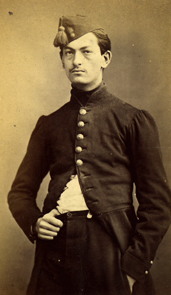
\includegraphics[width=\linewidth]{images/book3/b1-michel-levy.jpg}

{\scriptsize ميشيل–ليفي طالبًا، نحو 1862. ملك عام.}
\end{minipage}
\end{history}

يمكن إعطاء الموجتين الخارجتين من حبيبة تأخيرًا إضافيًا معلومًا بصفيحة ملحقة تُدخل فوق المقطع عند \ang{45} من المستقطِبين. وأشيعها مقطوعة لتُظهر الأحمر من الرتبة الأولى، أي تأخيرًا نحو \qty{540}{nm}. فإن توازى اتجاه الاهتزاز البطيء للحبيبة مع الاتجاه البطيء للصفيحة، تجتمع التأخيرات فيرتفع لون الحبيبة نحو رتبة واحدة؛ وإن توازى مع الاتجاه السريع، تتطرح فينخفض اللون. فالحبيبة الرمادية من \omterm{def:b1:optical-mineralogy:interference-colour}{الرتبة} الأولى بتأخير \qty{100}{nm} تصبح زرقاء من \omterm{def:b1:optical-mineralogy:interference-colour}{الرتبة} الثانية (\qty{640}{nm}) في أحد التوجهات، وبرتقالية من \omterm{def:b1:optical-mineralogy:interference-colour}{الرتبة} الأولى (\qty{440}{nm}) في الآخر؛ فالاختبار يبيّن أيّ الاتجاهين الاهتزازيين للحبيبة هو البطيء، وهي خاصية تُستعمل في تعيين \omterm{def:b1:rock-forming-minerals:mineral}{المعادن} المستطيلة.

\section{التعرّف على المعادن في الشريحة الرقيقة}

\begin{definition}[التوأم، والتوأمة المتعددة التركيب]\label{def:b1:optical-mineralogy:twin}
\emph{التوأم}\index{توأم (بلوري)} تداخل بلورتين أو أكثر من \omterm{def:b1:rock-forming-minerals:mineral}{المعدن} نفسه، تترابط شبكاتها بتناظر لا تملكه البلورة نفسها، كالانعكاس عبر مستوٍ (مستوى التوأمة). و\emph{التوأمة المتعددة التركيب}\index{التوأمة المتعددة التركيب} هي تكرار التوأمة على مستويات متوازية، يقسّم البلورة إلى صفائح رقيقة متوازية تتبادل توجّهاتها.
\end{definition}

بين \omterm{def:b1:field-lab-methods-1:microscope}{المستقطِبين المتقاطعين} تنطفئ صفائح \omterm{def:b1:optical-mineralogy:twin}{التوأمة المتعددة التركيب} بالتناوب: نصفها معتم حين يكون النصف الآخر مضيئًا، فتبدو البلورة مخطّطة. ويُظهر \omterm{def:b1:rock-forming-minerals:groups}{البلاجيوكلاز} هذه الخطوط دائمًا تقريبًا، فيميّزه فورًا عن الكوارتز وعن \omterm{def:b1:rock-forming-minerals:groups}{الفلسبار القلوي}؛ أما ميزته الأخرى، \omterm{def:b1:optical-mineralogy:relief}{البروز} المنخفض وألوان \omterm{def:b1:optical-mineralogy:interference-colour}{الرتبة} الأولى الرمادية إلى البيضاء، فيشاركهما فيها. وزوايا الانطفاء لمجموعتي الصفائح، المقاسة على جانبي مستوى التوأمة، تتوقف على تركيب \omterm{def:b1:rock-forming-minerals:groups}{البلاجيوكلاز}، وتعطي مخططات تلك الزوايا محتوى الأنورثيت فيه.

\begin{method}[تعيين معدن في الشريحة الرقيقة]\label{met:b1:optical-mineralogy:identify}
\begin{enumerate}
  \item في \omterm{def:b1:field-lab-methods-1:microscope}{الضوء المستقطَب المستوي}: لاحظ هل الحبيبة معتمة؛ ولونها وتعدّد ألوانها (أدِر المنضدة)؛ وبروزها، وعلى أي جهة من $1.54$ يقع معامل انكسارها (\omterm{def:b1:optical-mineralogy:relief}{خط بيك})؛ وشكلها وانشقاقاتها، والزاوية بين انشقاقين.
  \item بين \omterm{def:b1:field-lab-methods-1:microscope}{المستقطِبين المتقاطعين}: تحقّق هل تبقى معتمة (متساوية الخواص، أو مقطع عمودي على \omterm{def:b1:optical-mineralogy:optic-axis}{المحور البصري})؛ وبين حبيبات \omterm{def:b1:rock-forming-minerals:mineral}{المعدن} نفسه، جِد أعلى لون تداخل، واقرأ \omterm{def:b1:optical-mineralogy:birefringence}{الانكسار المزدوج} على \omterm{def:b1:optical-mineralogy:interference-colour}{مخطط ميشيل–ليفي} لسمك المقطع.
  \item قِس \omterm{def:b1:optical-mineralogy:extinction}{زاوية الانطفاء} على حبيبات تُظهر انشقاقًا أو استطالة؛ وابحث عن التوأمة (الخطوط المتعددة التركيب، والتوأمات البسيطة).
  \item قارن بجدول الخواص البصرية (\cref{tab:b1:optical-mineralogy:key}) وبالمعادن التي يمكن أن تحويها الصخرة (\cref{ch:b1:rock-forming-minerals}).
\end{enumerate}
\end{method}

\begin{table}[htbp]
\centering\footnotesize
\setlength{\tabcolsep}{3pt}
% ledger: hom:quartz-optics, hom:orthoclase-optics, hom:albite-optics, hom:anorthite-optics, hom:muscovite-optics, hom:biotite-optics, hom:hornblende-optics, hom:diopside-optics, hom:forsterite-optics, hom:fayalite-optics, hom:almandine-optics, hom:calcite-optics, hom:magnetite-optics
\begin{tabular}{@{}>{\raggedright\arraybackslash}p{2.0cm}>{\raggedright\arraybackslash}p{2.6cm}>{\raggedright\arraybackslash}p{2.3cm}>{\raggedright\arraybackslash}p{1.8cm}>{\raggedright\arraybackslash}p{3.0cm}>{\raggedright\arraybackslash}p{3.8cm}@{}}
\hline
\omterm{def:b1:rock-forming-minerals:mineral}{المعدن} & اللون في \omterm{def:b1:field-lab-methods-1:microscope}{الضوء المستقطَب المستوي} & المعاملات & \omterm{def:b1:optical-mineralogy:birefringence}{الانكسار المزدوج} & أعلى لون عند \qty{30}{\micro m} & سمات أخرى \\
\hline
الكوارتز & عديم اللون & 1.544--1.553 & 0.009 & أبيض من \omterm{def:b1:optical-mineralogy:interference-colour}{الرتبة} الأولى & لا انشقاق؛ ولا توأمات مرئية؛ \omterm{def:b1:optical-mineralogy:optic-axis}{أحادي المحور} \\
الأورثوكليز & عديم اللون، كثيرًا ما يكون عكِرًا & 1.518--1.525 & 0.005 & رمادي من \omterm{def:b1:optical-mineralogy:interference-colour}{الرتبة} الأولى & بروز سالب؛ توأمات بسيطة \\
\omterm{def:b1:rock-forming-minerals:groups}{البلاجيوكلاز} & عديم اللون & 1.526--1.590 & 0.008--0.013 & أبيض إلى أصفر باهت من \omterm{def:b1:optical-mineralogy:interference-colour}{الرتبة} الأولى & توأمة متعددة التركيب \\
المسكوفيت & عديم اللون & 1.552--1.618 & 0.035--0.042 & لامع من \omterm{def:b1:optical-mineralogy:interference-colour}{الرتبة} الثانية إلى الثالثة & انشقاق تام واحد؛ انطفاء مستقيم \\
البيوتيت & بنّي، أخضر & 1.565--1.696 & 0.04--0.07 & مُخفى بلونه هو & تعدّد ألوان قوي؛ انشقاق تام واحد \\
الهورنبلند & أخضر، بنّي & 1.675--1.695 & 0.020 & أزرق من \omterm{def:b1:optical-mineralogy:interference-colour}{الرتبة} الثانية & \omterm{def:b1:optical-mineralogy:pleochroism}{متعدد الألوان}؛ انشقاقان عند \ang{56}/\ang{124}؛ انطفاء \ang{15}--\ang{19} \\
الديوبسيد & عديم اللون & 1.664--1.694 & 0.030 & أصفر من \omterm{def:b1:optical-mineralogy:interference-colour}{الرتبة} الثانية & انشقاقان عند نحو \ang{87}/\ang{93}؛ انطفاء نحو \ang{38} \\
\omterm{def:b1:rock-forming-minerals:groups}{الأوليفين} & عديم اللون (المغنيسيوم) إلى أصفر باهت (الحديد) & 1.635--1.879 & 0.035--0.052 & نهاية \omterm{def:b1:optical-mineralogy:interference-colour}{الرتبة} الثانية إلى الثالثة & بروز مرتفع؛ شقوق غير منتظمة، دون انشقاق جيد \\
\omterm{def:b1:rock-forming-minerals:groups}{الجارنيت} & عديم اللون إلى وردي باهت & 1.830 (ألماندين) & \omterm{def:b1:optical-mineralogy:anisotropic}{متساوي الخواص} & أسود & بروز مرتفع جدًا؛ حدود سداسية أو ثمانية الأضلاع \\
الكالسيت & عديم اللون & 1.486--1.658 & 0.172 & أبيض عالي الرتبة & \omterm{def:b1:optical-mineralogy:relief}{البروز} يتغيّر عند الدوران؛ انشقاق معيني \\
المغنتيت & معتم & --- & --- & --- & أسود في الضوءين كليهما \\
\hline
\end{tabular}
\caption{الخواص البصرية \omterm{def:b1:rock-forming-minerals:mineral}{لمعادن} مكوِّنة للصخور شائعة في \omterm{def:b1:field-lab-methods-1:thin-section}{الشريحة الرقيقة}.
PPL: \omterm{def:b1:field-lab-methods-1:microscope}{الضوء المستقطَب المستوي}. يُقرأ أعلى لون على \omterm{def:b1:optical-mineralogy:interference-colour}{مخطط ميشيل–ليفي} عند $\Delta = \qty{30000}{nm}\times\delta$.}
\label{tab:b1:optical-mineralogy:key}
\end{table}

\begin{omfigure}
\setlength{\tabcolsep}{2pt}
\begin{tabular}{cc}
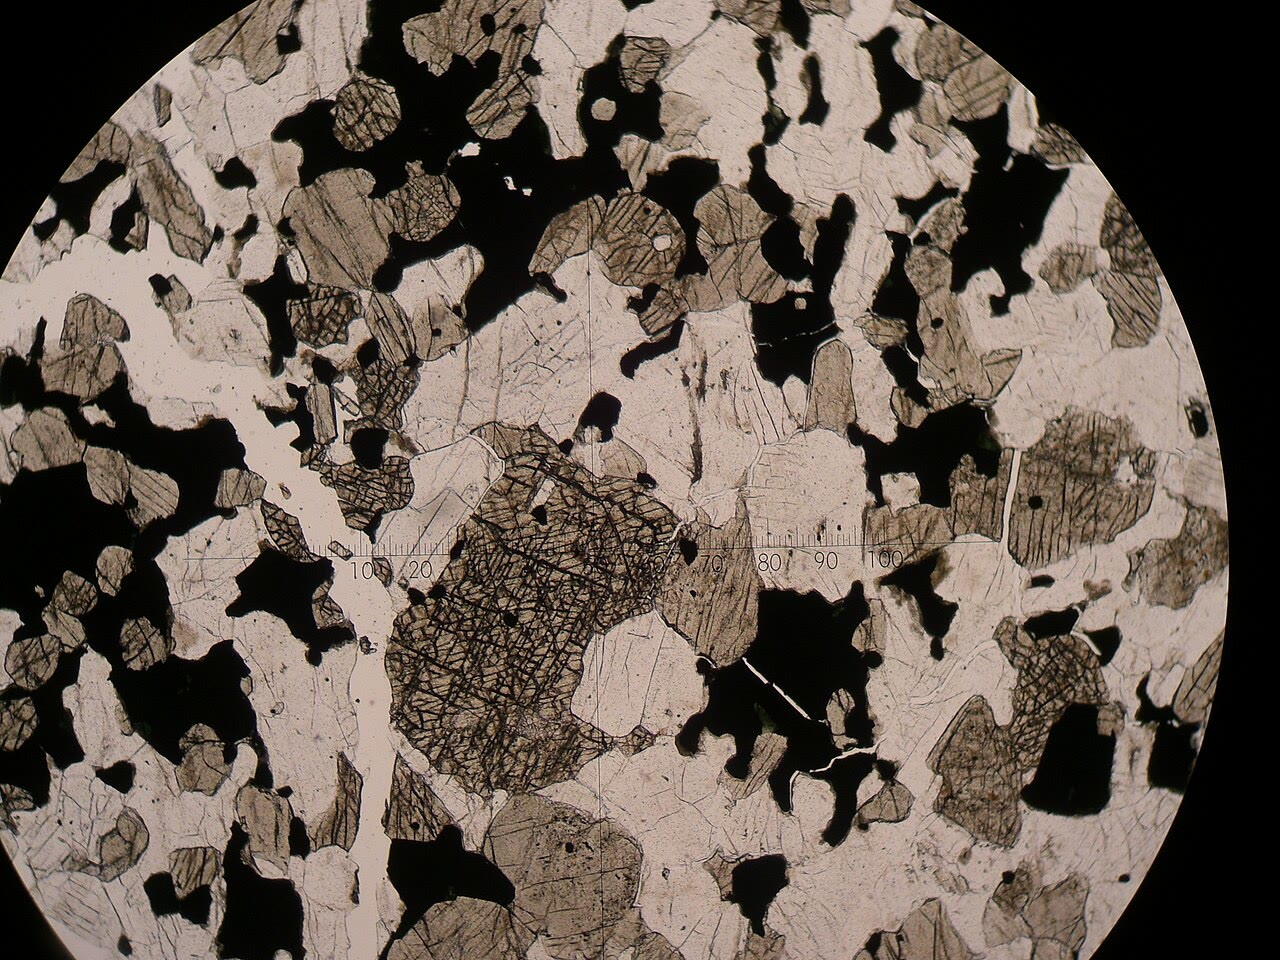
\includegraphics[width=0.485\linewidth]{images/book3/b1-gabbro-ppl.jpg} &
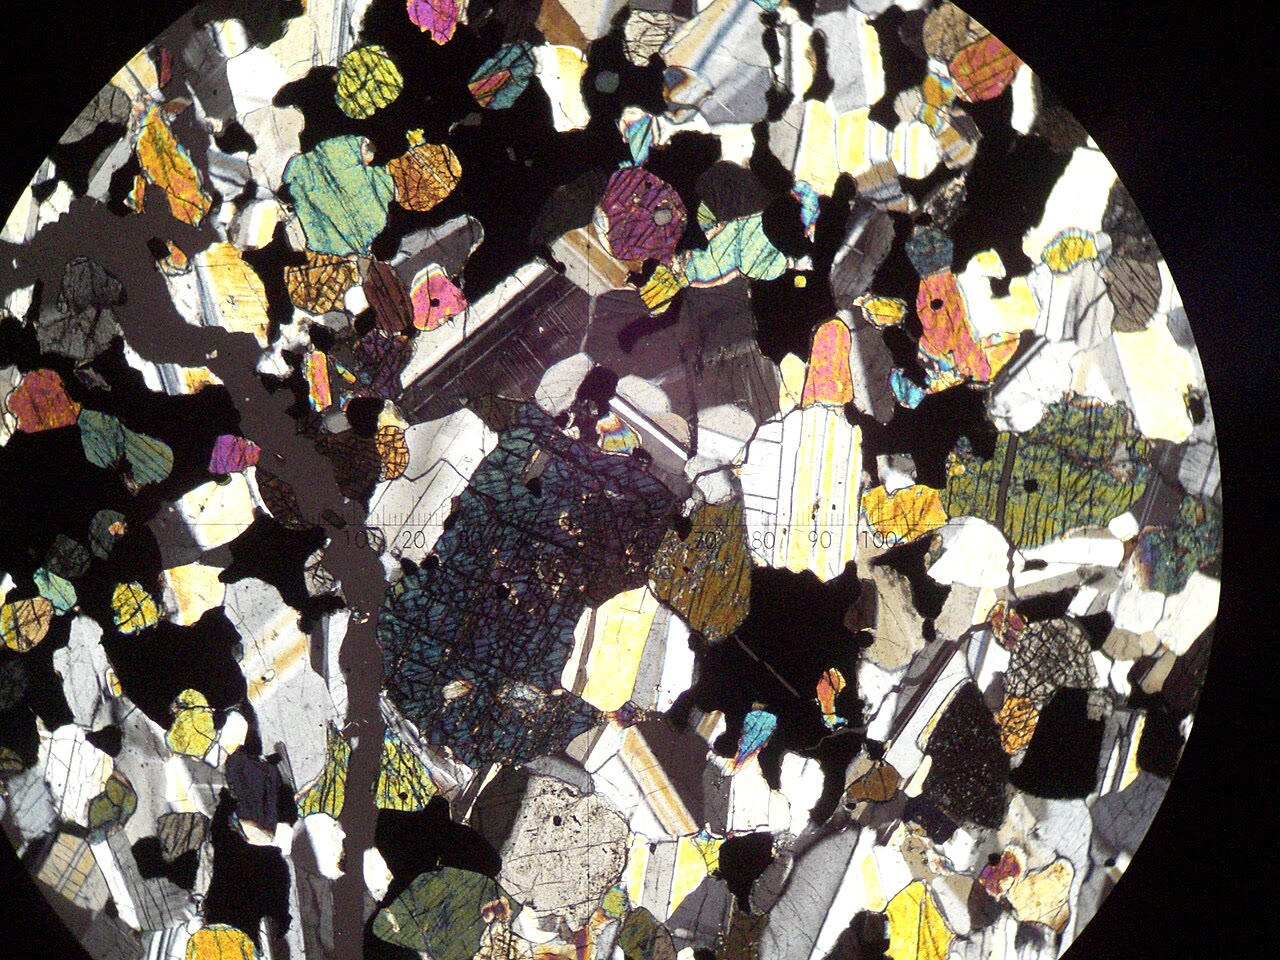
\includegraphics[width=0.485\linewidth]{images/book3/b1-gabbro-xpl.jpg} \\
{\small (أ) \omterm{def:b1:field-lab-methods-1:microscope}{الضوء المستقطَب المستوي}} & {\small (ب) \omterm{def:b1:field-lab-methods-1:microscope}{المستقطِبين المتقاطعين}} \\
\end{tabular}
% ledger: commons:gabbro-ppl, commons:gabbro-xpl

\medskip
{\small الحقل نفسه من الغابرو في \omterm{def:b1:field-lab-methods-1:thin-section}{الشريحة الرقيقة}. في \omterm{def:b1:field-lab-methods-1:microscope}{الضوء المستقطَب المستوي} (أ)، يكون \omterm{def:b1:rock-forming-minerals:groups}{البلاجيوكلاز} عديم اللون ذا بروز منخفض، وتكون حبيبات \omterm{def:b1:rock-forming-minerals:groups}{البيروكسين} \omterm{def:b1:rock-forming-minerals:groups}{والأوليفين} بنّية رمادية باهتة ذات بروز مرتفع وشقوق كثيفة، والخام المعتم أسود؛ والمقياس ميكرومتر في العدسة العينية. وبين \omterm{def:b1:field-lab-methods-1:microscope}{المستقطِبين المتقاطعين} (ب)، تتخطط صفائح \omterm{def:b1:rock-forming-minerals:groups}{البلاجيوكلاز} \omterm{def:b1:optical-mineralogy:twin}{بالتوأمة المتعددة التركيب}، وتلمع حبيبات \omterm{def:b1:rock-forming-minerals:groups}{البيروكسين} \omterm{def:b1:rock-forming-minerals:groups}{والأوليفين} بألوان \omterm{def:b1:optical-mineralogy:interference-colour}{الرتبة} الثانية، ويبقى الخام أسود. الصور ل\babelsublr{Chmee2}، بترخيص CC BY-SA 3.0 (\babelsublr{Wikimedia Commons}).}
\end{omfigure}

\begin{inthelab}[جلسة عند المجهر]
\begin{minipage}[t]{0.55\linewidth}\vspace{0pt}
تعمل عالِمة الصخور، حين تصف شريحة رقيقة جديدة، عليها أولًا بتكبير منخفض لترى النسيج \omterm{def:b1:rock-forming-minerals:mineral}{والمعادن} الرئيسية، ثم حبيبةً حبيبةً. وتسجّل لكل \omterm{def:b1:rock-forming-minerals:mineral}{معدن} ملاحظات الطريقة السابقة، وتقدّر نسبته في الشريحة، وتلاحظ كيف تتلامس الحبيبات: أيّها تبلّر أولًا، وأيّها يملأ الفراغات المتبقية، وأيّها يحلّ محل غيره. وتُجرى القياسات الضوئية بمنضدة مدرّجة بالدرجات ومع صفيحة ملحقة؛ أما التراكيب، حين تهمّ، فتُقاس لاحقًا بمسبار دقيق على الشريحة نفسها. ويعمل مختبر التدريس بالطريقة نفسها: مجهر لكل طالب، وعلبة من الشرائح المرجعية \omterm{def:b1:rock-forming-minerals:mineral}{لمعادن} معلومة بجانبه.
\end{minipage}\hfill
\begin{minipage}[t]{0.42\linewidth}\vspace{0pt}
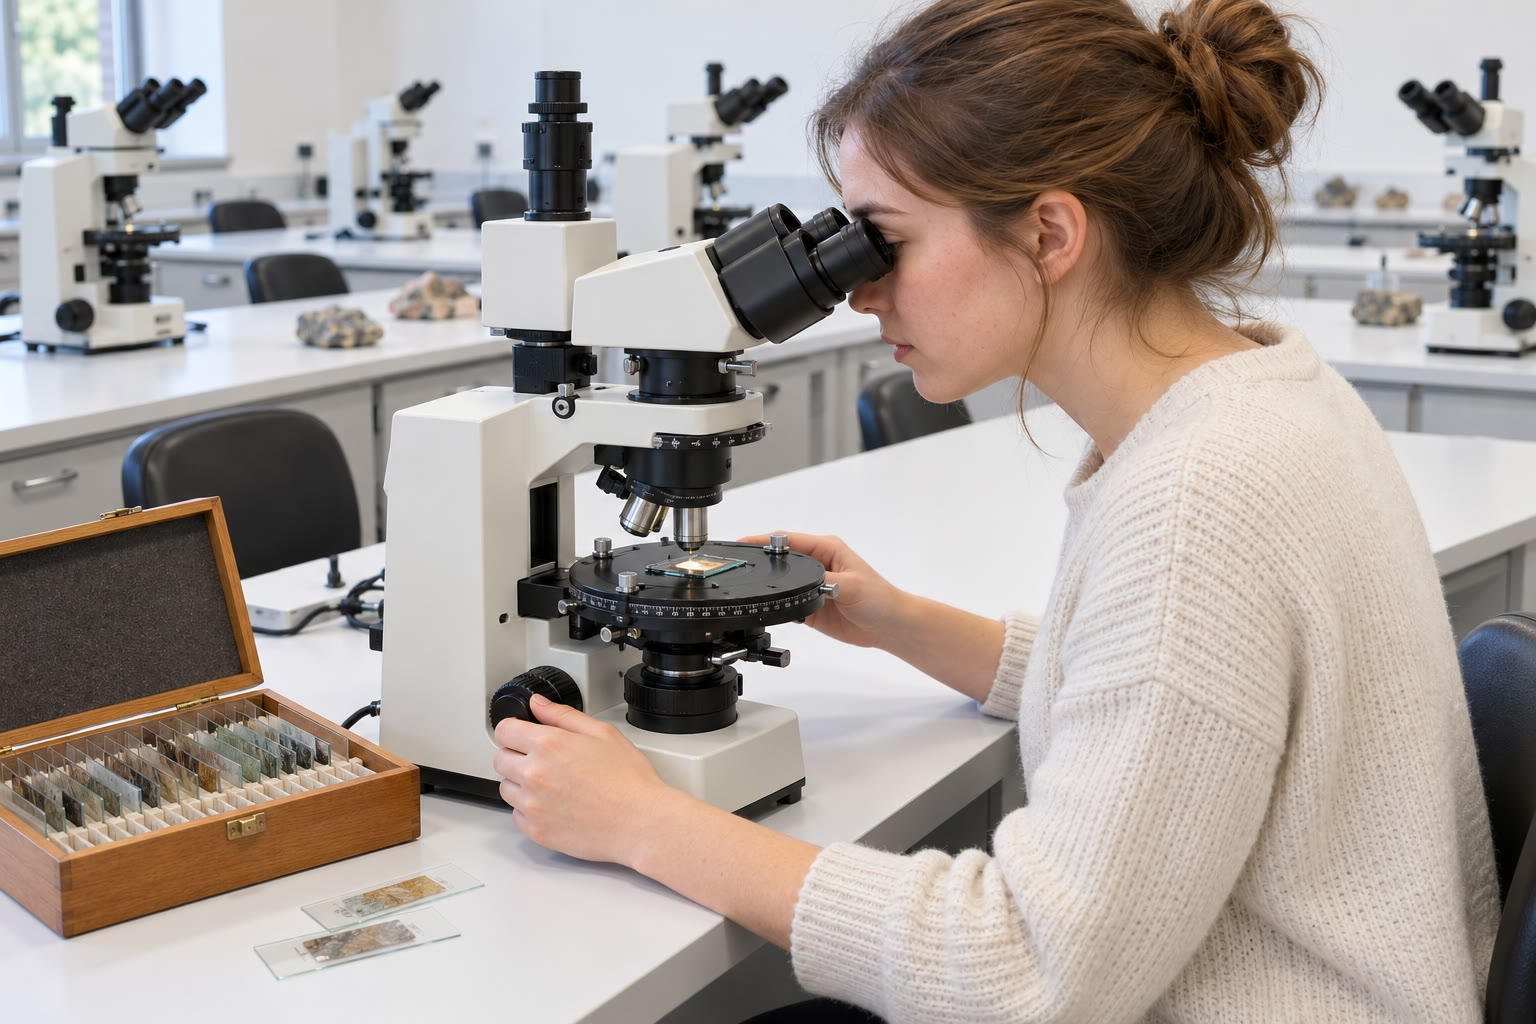
\includegraphics[width=\linewidth]{images/book3/ai/b1-microscope-student.jpg}

{\scriptsize طالب عند \omterm{def:b1:field-lab-methods-1:microscope}{المجهر المستقطِب} في مختبر تدريس (رسم توضيحي مُولَّد بالذكاء الاصطناعي).}
\end{minipage}
\end{inthelab}

\section{التمارين}

\begin{exercise}[$\star$]\label{exo:b1:optical-mineralogy:1}
احسب أكبر تأخير للكوارتز ($\delta = 0.009$) وللكالسيت ($\delta = 0.172$) في مقطع سمكه \qty{30}{\micro m}. وباستعمال \omterm{def:b1:optical-mineralogy:interference-colour}{مخطط ميشيل–ليفي}، صف لون كل منهما.
% ledger: hom:quartz-optics, hom:calcite-optics
\end{exercise}

\begin{exercise}[$\star$]\label{exo:b1:optical-mineralogy:2}
تُدار حبيبة على المنضدة بين \omterm{def:b1:field-lab-methods-1:microscope}{المستقطِبين المتقاطعين}. احسب $I/I_0$، ككسر من قيمته العظمى، عند $\theta = 0$، و\ang{22.5}، و\ang{45}، و\ang{67.5}، و\ang{90} من \omterm{def:b1:optical-mineralogy:extinction}{موضع الانطفاء}.
\end{exercise}

\begin{exercise}[$\star$]\label{exo:b1:optical-mineralogy:3}
اشرح لماذا يبقى \omterm{def:b1:rock-forming-minerals:groups}{الجارنيت} أسود بين \omterm{def:b1:field-lab-methods-1:microscope}{المستقطِبين المتقاطعين} مهما كان وضع المنضدة، ولماذا قد تفعل حبيبة الكوارتز ذلك أيضًا. كيف تميّز بينهما في \omterm{def:b1:field-lab-methods-1:microscope}{الضوء المستقطَب المستوي}؟
\end{exercise}

\begin{exercise}[$\star$]\label{exo:b1:optical-mineralogy:4}
رتّب بحسب \omterm{def:b1:optical-mineralogy:relief}{البروز}، في وسط تثبيت معامله $1.54$، الأورثوكليز ($n$ نحو $1.52$)، والكوارتز ($1.55$)، والفورستيريت ($1.65$)، والألماندين ($1.83$). أيّها له بروز سالب؟ وفي أي اتجاه يتحرك \omterm{def:b1:optical-mineralogy:relief}{خط بيك} عند رفع البؤرة؟
% ledger: hom:orthoclase-optics, hom:quartz-optics, hom:forsterite-optics, hom:almandine-optics
\end{exercise}

\begin{exercise}[$\star\star$]\label{exo:b1:optical-mineralogy:5}
في مقطع \qty{30}{\micro m}، تُظهر حبيبات \omterm{def:b1:rock-forming-minerals:mineral}{معدن} أخضر \omterm{def:b1:optical-mineralogy:pleochroism}{متعدد الألوان}، له انشقاقان عند \ang{56} و\ang{124}، أعلى ما يُظهره أزرق من الرتبة الثانية، يُقرأ على المخطط $\Delta = \qty{650}{nm}$. احسب انكساره المزدوج وسمِّ \omterm{def:b1:rock-forming-minerals:mineral}{المعدن} باستعمال \cref{tab:b1:optical-mineralogy:key}.
\end{exercise}

\begin{exercise}[$\star\star$]\label{exo:b1:optical-mineralogy:6}
باستعمال \cref{prop:b1:optical-mineralogy:relief} مع $n_m = 1.54$ و$i = \ang{30}$، احسب الانحراف عند حافة حبيبة كوارتز ($n = 1.553$) وحبيبة فورستيريت ($n = 1.651$)، بالدرجات، ونسبة الاثنين. وتحقّق من الثانية بقانون سنل بصورته التامة.
\end{exercise}

\begin{exercise}[$\star\star$]\label{exo:b1:optical-mineralogy:7}
صفيحة حمراء من الرتبة الأولى لها $\Delta = \qty{540}{nm}$. توضع حبيبة كوارتز $\Delta = \qty{270}{nm}$ عند \ang{45} مع إدخال الصفيحة. ما التأخيران الكليان الممكنان، والألوان التي يعطيانها على المخطط؟ وأيّ توجّه يجعل الاتجاهين البطيئين متوازيين؟
\end{exercise}

\begin{exercise}[$\star\star$]\label{exo:b1:optical-mineralogy:8}
عند حافته المتناقصة، تنحسر حبيبة فايالايت ($\delta = 0.052$) من \qty{30}{\micro m} إلى الصفر. كم من الألوان الأرجوانية المحمّرة، التي تنهي الرتب عند 542 و\num{1074} و\qty{1605}{nm}، تظهر كأهداب ملوّنة بين الحافة والجزء الكامل السمك من الحبيبة؟
% ledger: hom:fayalite-optics
\end{exercise}

\begin{exercise}[$\star\star$]\label{exo:b1:optical-mineralogy:9}
على عدة حبيبات مستطيلة ذات انشقاق جيد واحد، يقيس جيولوجي زوايا الانطفاء قدرها \ang{0} و\ang{21} و\ang{36} و\ang{37} بين أثر الانشقاق واتجاه الاهتزاز البطيء. لماذا تختلف القيم؟ وهل \omterm{def:b1:rock-forming-minerals:mineral}{المعدن} أرجح أن يكون ديوبسيدًا أم هورنبلندًا؟
% ledger: hom:diopside-optics, hom:hornblende-optics
\end{exercise}

\begin{exercise}[$\star\star\star$]\label{exo:b1:optical-mineralogy:10}
أعد برهان \cref{thm:b1:optical-mineralogy:intensity} والمحلِّل موازٍ للمستقطِب، وبيّن أن
$I_\parallel = I_0\bigl(1 - \sin^2 2\theta\sin^2(\pi\Delta/\lambda)\bigr)$.
أيّ لون تُظهره حبيبة $\Delta = \qty{550}{nm}$ عند \ang{45} بين مستقطِبين متوازيين؟
\end{exercise}

\begin{exercise}[$\star\star\star$]\label{exo:b1:optical-mineralogy:11}
لحبيبة كالسيت $\Delta = \qty{5000}{nm}$، يتلاشى العامل $\sin^2(\pi\Delta/\lambda)$ كلما كان $\Delta/\lambda$ عددًا صحيحًا. (أ) كم مرة يتلاشى بين \num{400} و\qty{700}{nm}؟ (ب) بيّن أنه قرب $\lambda = \qty{550}{nm}$ يبعد صفران متتاليان نحو $\lambda^2/\Delta$، واحسبه. (ج) اشرح لماذا تبدو الحبيبة أبيض تقريبًا.
\end{exercise}

\begin{exercise}[$\star\star\star$]\label{exo:b1:optical-mineralogy:12}
بيّن أنه، متوسطًا على دورة كاملة للمنضدة، تمرّر حبيبة بين \omterm{def:b1:field-lab-methods-1:microscope}{المستقطِبين المتقاطعين} القدر $\frac12 I_0\sin^2(\pi\Delta/\lambda)$. يُقدّر جيولوجي الانكسارات المزدوجة من أعلى لون لكل \omterm{def:b1:rock-forming-minerals:mineral}{معدن}، مفترضًا \qty{30}{\micro m}، في مقطع سمكه في الحقيقة \qty{25}{\micro m}. بأي معامل تكون كل قيمه خاطئة، وفي أي اتجاه؟
\end{exercise}

\section{مسألة: تعيين معادن شريحة رقيقة مجهولة}

\begin{problem}[{مسألة نهاية الأسبوع --- ملاحظة البروز وتعدّد الألوان وألوان التداخل، وقياس سمك مقطع بالكوارتز، وتسمية معادنه}]
\label{pb:b1:optical-mineralogy:1}
% values: calc/ch08.py; optical data: ledger hom:*-optics
% ledger: hom:quartz-optics, hom:diopside-optics, hom:forsterite-optics, hom:albite-optics, hom:anorthite-optics, hom:hornblende-optics, hom:biotite-optics
\omterm{def:b1:field-lab-methods-1:thin-section}{الشريحة الرقيقة} لصخر ناري مجهول، مثبّتة في راتنج معامله $1.540$، يُقال إن سمكها \qty{30}{\micro m}. تحوي خمسة \omterm{def:b1:rock-forming-minerals:mineral}{معادن}، مُسمّاة من A إلى E. استعمل جدول الخواص البصرية في الفصل، \omterm{def:b1:optical-mineralogy:interference-colour}{ومخطط ميشيل–ليفي}، والقيم التالية: الكوارتز $n_\omega = 1.544$، و$n_\varepsilon = 1.553$؛ والديوبسيد $n_\alpha = 1.664$، و$n_\beta = 1.672$، و$n_\gamma = 1.694$.

\medskip
\noindent\textbf{الجزء الأول --- \omterm{def:b1:field-lab-methods-1:microscope}{الضوء المستقطَب المستوي}.}
\begin{enumerate}
  \item \omterm{def:b1:rock-forming-minerals:mineral}{المعدن} A عديم اللون، وحدود حبيباته يصعب رؤيتها. \omterm{def:b1:rock-forming-minerals:mineral}{والمعدن} B عديم اللون، ذو حواف داكنة قوية، وانشقاقان يلتقيان عند
        نحو \ang{87}. أيّهما له \omterm{def:b1:optical-mineralogy:relief}{البروز} الأعلى؟
  \item \omterm{def:b1:rock-forming-minerals:mineral}{للمعدن} A، معتبرًا إياه كوارتزًا، وللمعدن B، معتبرًا إياه ديوبسيدًا، احسب $|n - n_m|$ باستعمال متوسط المعاملات الرئيسية لكل منهما.
  \item باستعمال \cref{prop:b1:optical-mineralogy:relief}، احسب نسبة الانحرافين عند حافتيهما لميل الحد نفسه.
  \item عند رفع البؤرة يتحرك \omterm{def:b1:optical-mineralogy:relief}{خط بيك} \omterm{def:b1:rock-forming-minerals:mineral}{للمعدن} B نحو الحبيبة. ماذا يدل ذلك؟
  \item يتحول \omterm{def:b1:rock-forming-minerals:mineral}{المعدن} C من أصفر باهت إلى بنّي داكن عند دوران المنضدة، ويكون أشدّ قتامة حين يقع انشقاقه الوحيد على امتداد المستقطِب. سمِّ الخاصية \omterm{def:b1:rock-forming-minerals:mineral}{والمعدن}.
  \item \omterm{def:b1:rock-forming-minerals:mineral}{المعدن} D عديم اللون، ذو بروز منخفض، في صفائح طويلة؛ \omterm{def:b1:rock-forming-minerals:mineral}{والمعدن} E أخضر إلى أصفر، \omterm{def:b1:optical-mineralogy:pleochroism}{متعدد الألوان}، له انشقاقان عند \ang{124}. ماذا تقترح الزاوية بالنسبة إلى E؟
\end{enumerate}

\medskip
\noindent\textbf{الجزء الثاني --- سمك المقطع.}
\begin{enumerate}[resume]
  \item ما أكبر تأخير للكوارتز في مقطع سمكه \qty{30}{\micro m} بالضبط؟ وما لونه؟
  \item لماذا يجب البحث عن أكبر تأخير بين حبيبات كثيرة من A، بدلًا من قياسه على حبيبة واحدة منها؟
  \item أعلى لون تُظهره حبيبات A هو أصفر باهت من \omterm{def:b1:optical-mineralogy:interference-colour}{الرتبة} الأولى؛ ومقارِن الإسفين الكوارتزي يعطي تأخيرها \qty{342}{nm}. احسب \omterm{def:b1:cross-sections:thickness}{السمك الحقيقي} للمقطع.
  \item بكم في المئة يكون المقطع أسمك مما ينبغي؟
  \item عند $\lambda = \qty{550}{nm}$ وعلى \ang{45} من الانطفاء، احسب $I/I_0$ لحبيبة الكوارتز هذه، ولحبيبة الكوارتز نفسها في مقطع سمكه \qty{30}{\micro m}.
  \item احسب مجال التأخيرات \omterm{def:b1:rock-forming-minerals:mineral}{للمعدن} D، معتبرًا إياه \omterm{def:b1:rock-forming-minerals:groups}{البلاجيوكلاز} ($\delta = 0.008$ إلى $0.013$)، في هذا المقطع، وبيّن هل تبقى ألوانه في \omterm{def:b1:optical-mineralogy:interference-colour}{الرتبة} الأولى.
\end{enumerate}

\medskip
\noindent\textbf{الجزء الثالث --- \omterm{def:b1:optical-mineralogy:birefringence}{الانكسار المزدوج} \omterm{def:b1:rock-forming-minerals:mineral}{للمعدن} B.}
\begin{enumerate}[resume]
  \item اللون الأعلى \omterm{def:b1:rock-forming-minerals:mineral}{للمعدن} B أزرق يُقرأ $\Delta = \qty{1140}{nm}$. في أي رتبة هو؟
  \item احسب \omterm{def:b1:optical-mineralogy:birefringence}{الانكسار المزدوج} \omterm{def:b1:rock-forming-minerals:mineral}{للمعدن} B بالسمك الذي وجدته في السؤال 9.
  \item أيّ انكسار مزدوج كان سيُوجد بافتراض \qty{30}{\micro m}؟ وأي \omterm{def:b1:rock-forming-minerals:mineral}{معدن} عديم اللون ذي بروز مرتفع كان سيوحيه ذلك، ولماذا لا مكان له في صخرة فيها كوارتز (انظر \ce{Mg2SiO4 + SiO2 -> 2 MgSiO3})؟
  \item قارن نتيجة السؤال 14 بالجدول، مع \omterm{def:b1:optical-mineralogy:relief}{البروز} وانشقاقات B، واستنتج.
  \item ما اللون الذي يُظهره \omterm{def:b1:rock-forming-minerals:mineral}{المعدن} B على الأكثر في مقطع صحيح سمكه \qty{30}{\micro m}؟
  \item يُطحن المقطع حتى يصبح \qty{30}{\micro m}. بكم يجب تقليل سمكه، وما أعلى لون للكوارتز عندئذٍ؟
\end{enumerate}

\medskip
\noindent\textbf{الجزء الرابع --- الانطفاء والتوأمة.}
\begin{enumerate}[resume]
  \item تنقسم صفائح D إلى مخطّطات متوازية تنطفئ بالتناوب. سمِّ الظاهرة \omterm{def:b1:rock-forming-minerals:mineral}{والمعدن}.
  \item تنطفئ مخطّطات صفيحة واحدة عند \ang{27} و\ang{28} على جانبي مستوى التوأمة. ماذا تعطي مثل هذه الزوايا، إذا قيست على صفائح كثيرة، عند مقارنتها بالمخططات المنشورة؟
  \item أعلى زاوية انطفاء بين انشقاقات E واتجاه اهتزازه البطيء هي \ang{17}. سمِّ E.
  \item احسب أكبر تأخير \omterm{def:b1:rock-forming-minerals:mineral}{للمعدن} E في هذا المقطع، واللون الذي يُظهره.
  \item تبقى حبيبة من B معتمة خلال دورة كاملة. اشرح كيف يمكن أن تكون \omterm{def:b1:rock-forming-minerals:mineral}{المعدن} نفسه الذي تُظهر حبيباته الأخرى ضوءًا.
  \item اذكر \omterm{def:b1:rock-forming-minerals:mineral}{المعادن} A إلى E، وأيّ صنف من الصخور تكوّن.
  \item ما \omterm{def:b1:cross-sections:thickness}{السمك الحقيقي} للمقطع بالميكرومتر؟
\end{enumerate}
\end{problem}
